\section{Przetwarzanie i wykorzystywanie danych geograficznych - OpenStreetMap}

\par \emph{OpenStreetMap}, znane skrótowo jako \emph{OSM}, to projekt tworzenia mapy, który zaangażowuje społeczność. Jego głównym celem jest stworzenie darmowej, otwartej i edytowalnej mapy całego świata. Dane zgromadzone w ramach tego projektu są ogólnie dostępne, głównie na podstawie licencji \emph{Open Database License}. Warto jednak zaznaczyć, że nie wszystkie elementy projektu podlegają tej samej licencji. Niektóre fragmenty \emph{OSM} korzystają z innych licencji, takich jak na przykład \emph{Creative Commons Attribution-ShareAlike}.

\par Projekt ten jest tworzony przez wolontariuszy, którzy dodają i aktualizują dane, z których każdy może skorzystać, zmodyfikować, jak i dzielić się, oczywiście, przy zachowaniu zasad zawartych w licencji. Poza samymi informacjami o drogach, można również znaleźć inne szczegółowe dane, takie jak na przykład: ograniczenia prędkości, granice administracyjne, czy punkty zainteresowania\english{Point of Interest}. Wszystkie te cechy przyczyniły się do ogromnej popularności \emph{OSM} i wykorzystaniu ich w projektach, gdzie inne mapy ograniczone licencjami się nie nadają.

\par Mapy te są dostępne do pobrania na oficjalnej stronie\cite{OPEN_STREET_MAPS_SITE}, jednak dużo bardziej zaawansowanym narzędziem jest \emph{overpass turbo}\cite{OVERPASS_TURBO_SITE}, będący interfejsem dla \emph{Overpass API}. Pozwala on, przy wykorzystaniu specjalnego języka kwerend\footnote{Overpass QL}, na wyeksportowanie odpowiednio przefiltrowanych i transformowanych danych dotyczących regionu, który nas interesuje. Dzięki niemu możemy pobrać tylko i wyłącznie drogi znajdujące się w danej miejscowości, w przeciwieństwie do oficjalnej strony, gdzie wskazujemy  tak zwany \emph{bounding box}, dzięki któremu otrzymamy wszystkie informacje map z danego regionu. Narzędzie to naturalnie oferuje również wiele innych możliwości.

\par Otrzymane w ten sposób pliki \emph{OSM} można dalej analizować i przetwarzać, wykorzystując rozszerzenie \emph{PostGis}\cite{POSTGIS_SITE} do bazy danych \emph{PostgreSQL}\cite{POSTGRESQL_SITE}. Rozszerzenie to pozwala na przechowywanie danych geograficznych w standardowym formacie \emph{OGC}\footnote{Open Geospatial Consortium}. Dodatkowo oferuje szeroki wachlarz funkcji przestrzennych pozwalających na dokonanie obliczeń odległości, przecięć, powierzchni oraz złączeń przestrzennych. Niestety jednak nie pozwala ono, na wyznaczenie trasy między dwoma punktami. W tym celu można wykorzystać \emph{pgRouting}\cite{PGROUTING_SITE}.

\begin{figure}
    \centering
    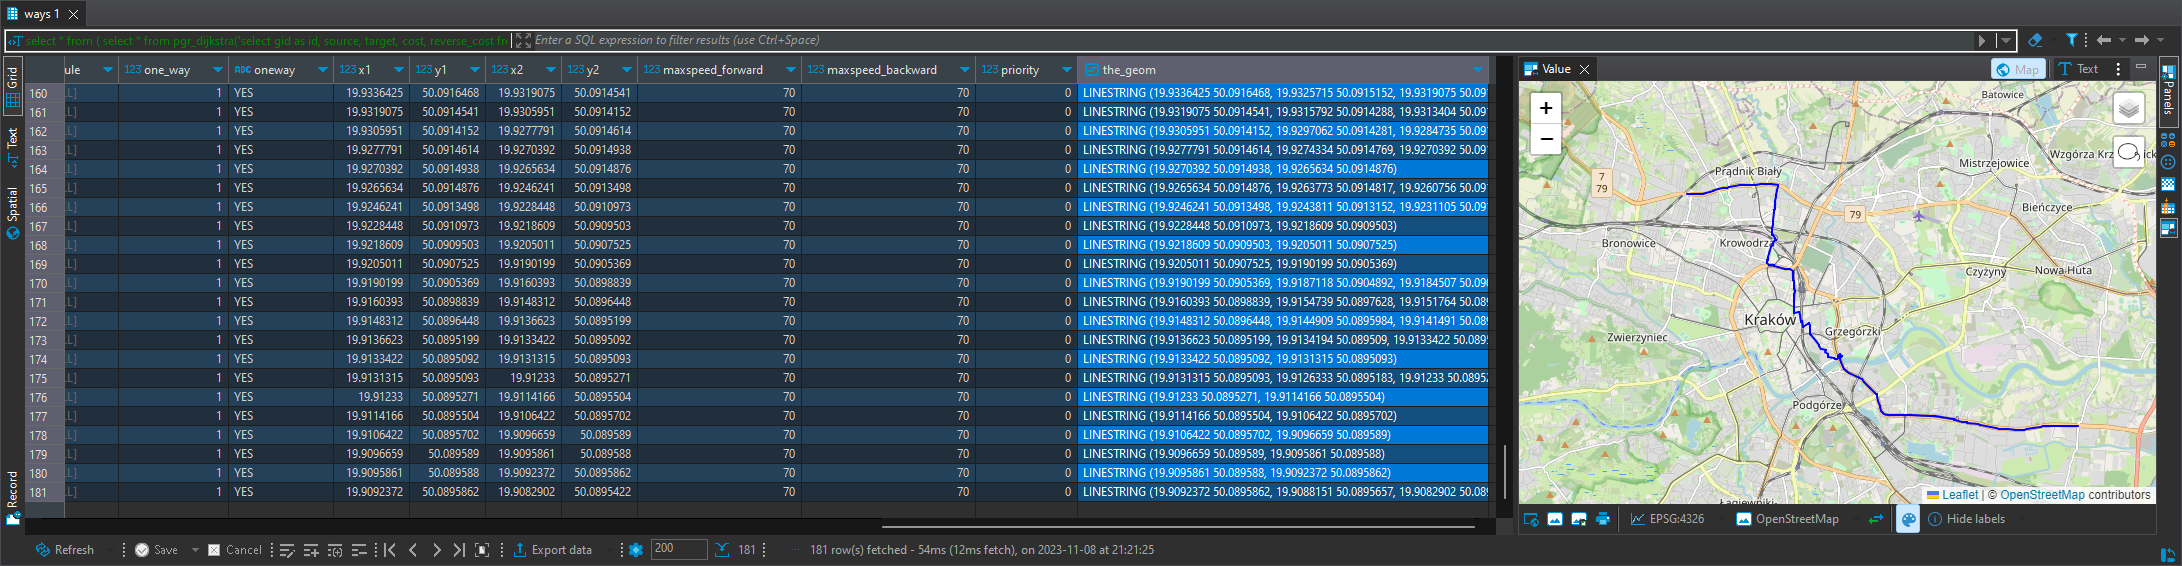
\includegraphics[width=\linewidth]{DBeaver OSM Example}
    \caption{Przykładowa trasa \emph{OSM} w Krakowie wyświetlana przy wykorzystaniu \emph{DBeaver}}
    \label{fig:dbeaverOSMExample}
    \source{Opracowanie Własne}
\end{figure}